\section{系統設計}

\subsection{機器人硬體設計}
機器人的車體部分,我們沿用MIT Duckietown之車架壓克力板,但是為了更好的載重量我們將馬達改成具有編碼器之馬達,除了增加穩定性與馬力以外,未來也可加入Wheel Odometry之功能提供更完整的SLAM。主控板部分我們使用Nvidia發行之Jetson Nano,具有強大的圖形運算能力,能為深度學習的Model提供更可靠的運算處理。為了能夠定位以及辨識物體,我們在車上加上Pozyx公司推出的UWB裝置,以及Intel RealSense的D435深度相機。前者能夠提供3D Pose定位後者能夠提供RGBD之深度影像有利於視覺辨識與計算物體相對位置。


\begin{figure}[h] % h means put this image here
  \centering
    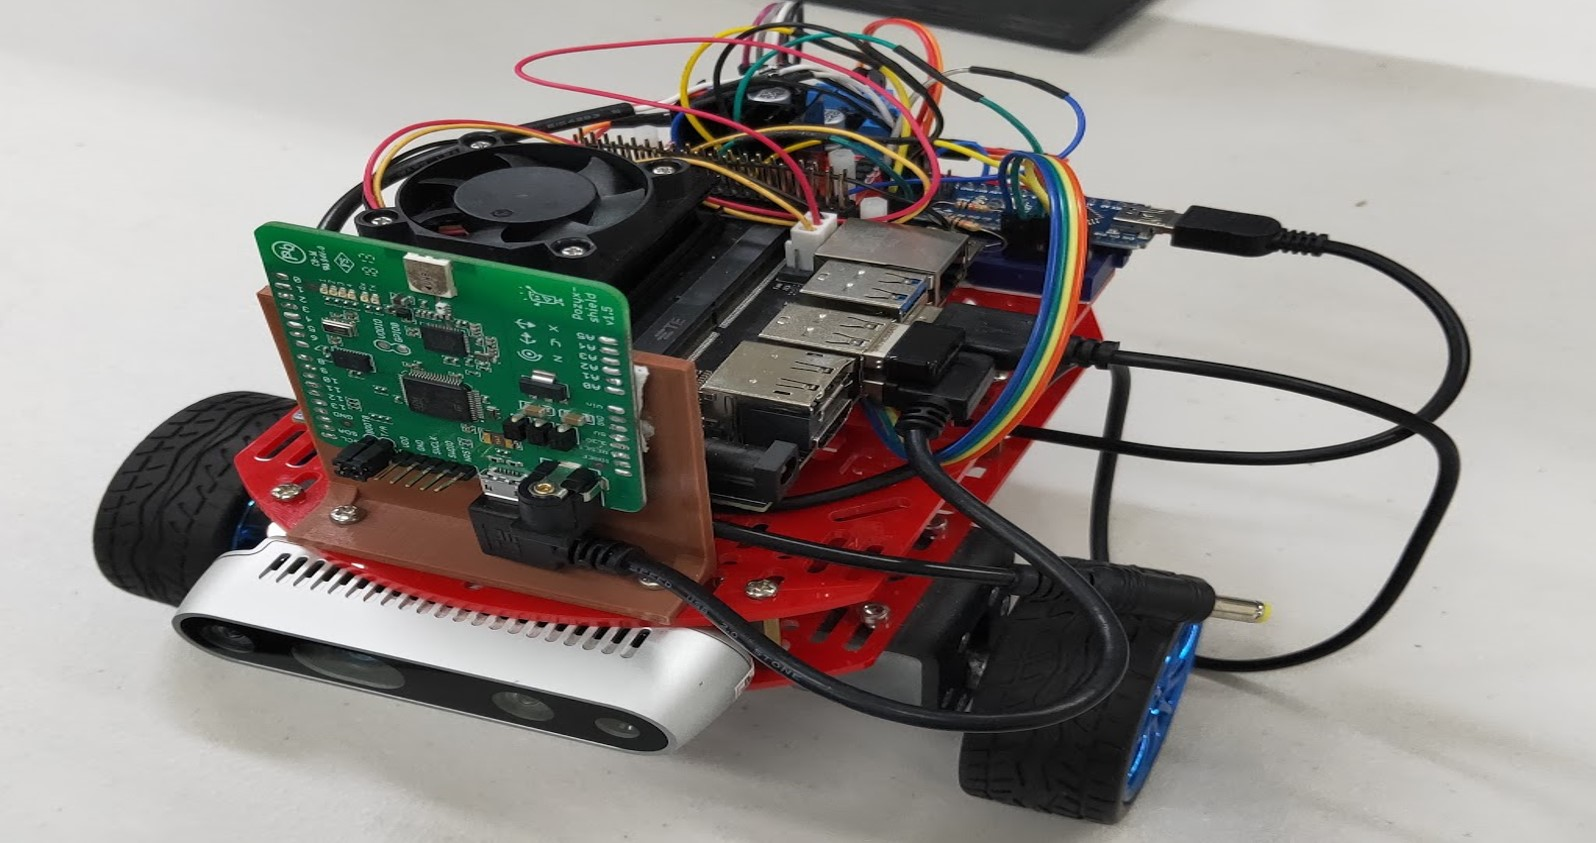
\includegraphics[width=0.8\columnwidth]{images/jetson-car_2.jpg}	
      \caption{核災應變機器人之硬體設計}
    \label{figure:car2}
\end{figure}

\subsection{機器人作業系統}
在機器人上運行的系統,我們安裝Ubuntu18.04與ROS Melodic。ROS(Robot Operating System)是專為機器人軟體開發所設計出來的一套電腦作業系統架構。它是一個開源的元級作業系統,提供類似於作業系統的服務,包括硬體抽象描述、底層驅動程序管理、共用功能的執行、程序間消息傳遞、程序發行包管理,它也提供一些工具和庫用於獲取、建立、編寫和執行多機融合的程序。
利用ROS我們能夠快速建立各種Node並利用Publisher與Subscriber互相傳送資訊。

\subsection{機器人定位與移動}
我們用pypozyx的函式庫取得Tag Pose並且Publish至ROS topic,另一個Node將每個Pose記錄下來後,可在地圖上畫出一個行進軌跡,方便搜尋到物品之後進行後續的動作。
機器人的移動是利用ROS的Joy Package搭配ROS Serial將car command傳送至Arduino驅動馬達,達到利用Joystick控制車子行進之功能。

\subsection{機器人視覺與物品定位}
抽取D435之RGB影像後,首先使用MobileNet-SSD進行物品辨識,我們將搜索到的物品在畫面中標出Bounding Box之後,利用Depth資料以及CameraInfo將影像投影至三維空間,標出物品相對位置以後,利用TF函式乘上Pozyx的Pose資訊,

\begin{figure}[h] % h means put this image here
  \centering
    
\includegraphics[width=0.8\columnwidth]{images/tf.png}	
      \caption{物品座標轉換}
    \label{figure:tf}
\end{figure}